\subsection{Current operating evidence and the forecast handoff}

The operational decomposition developed by Team~4 is retained, but its
empirical inputs are refreshed with Barrick's Q1 and Q2 2026 mine-statistics
tables. The current evidence is deliberately limited to physical production,
ore processed, processed grade, recovery and Cost of Sales. The standalone
article's NSS curve, option inversion, GBM paths and illustrative stochastic
EBITDA valuation are not inputs to this thesis valuation.

Figures~\ref{fig:team4-production-qoq} and
\ref{fig:team4-cost-qoq} compare the two available 2026 quarters for the
eight-mine analytical perimeter. The selected mines produced 622 attributable
koz in Q1 and 711 koz in Q2; the difference from Barrick's company totals of
719 and 796 koz is expected because the company totals include other
operations. Company-wide Cost of Sales was USD~1,922/oz in Q1 and
USD~1,993/oz in Q2.

\begin{figure}[htbp]
    \centering
    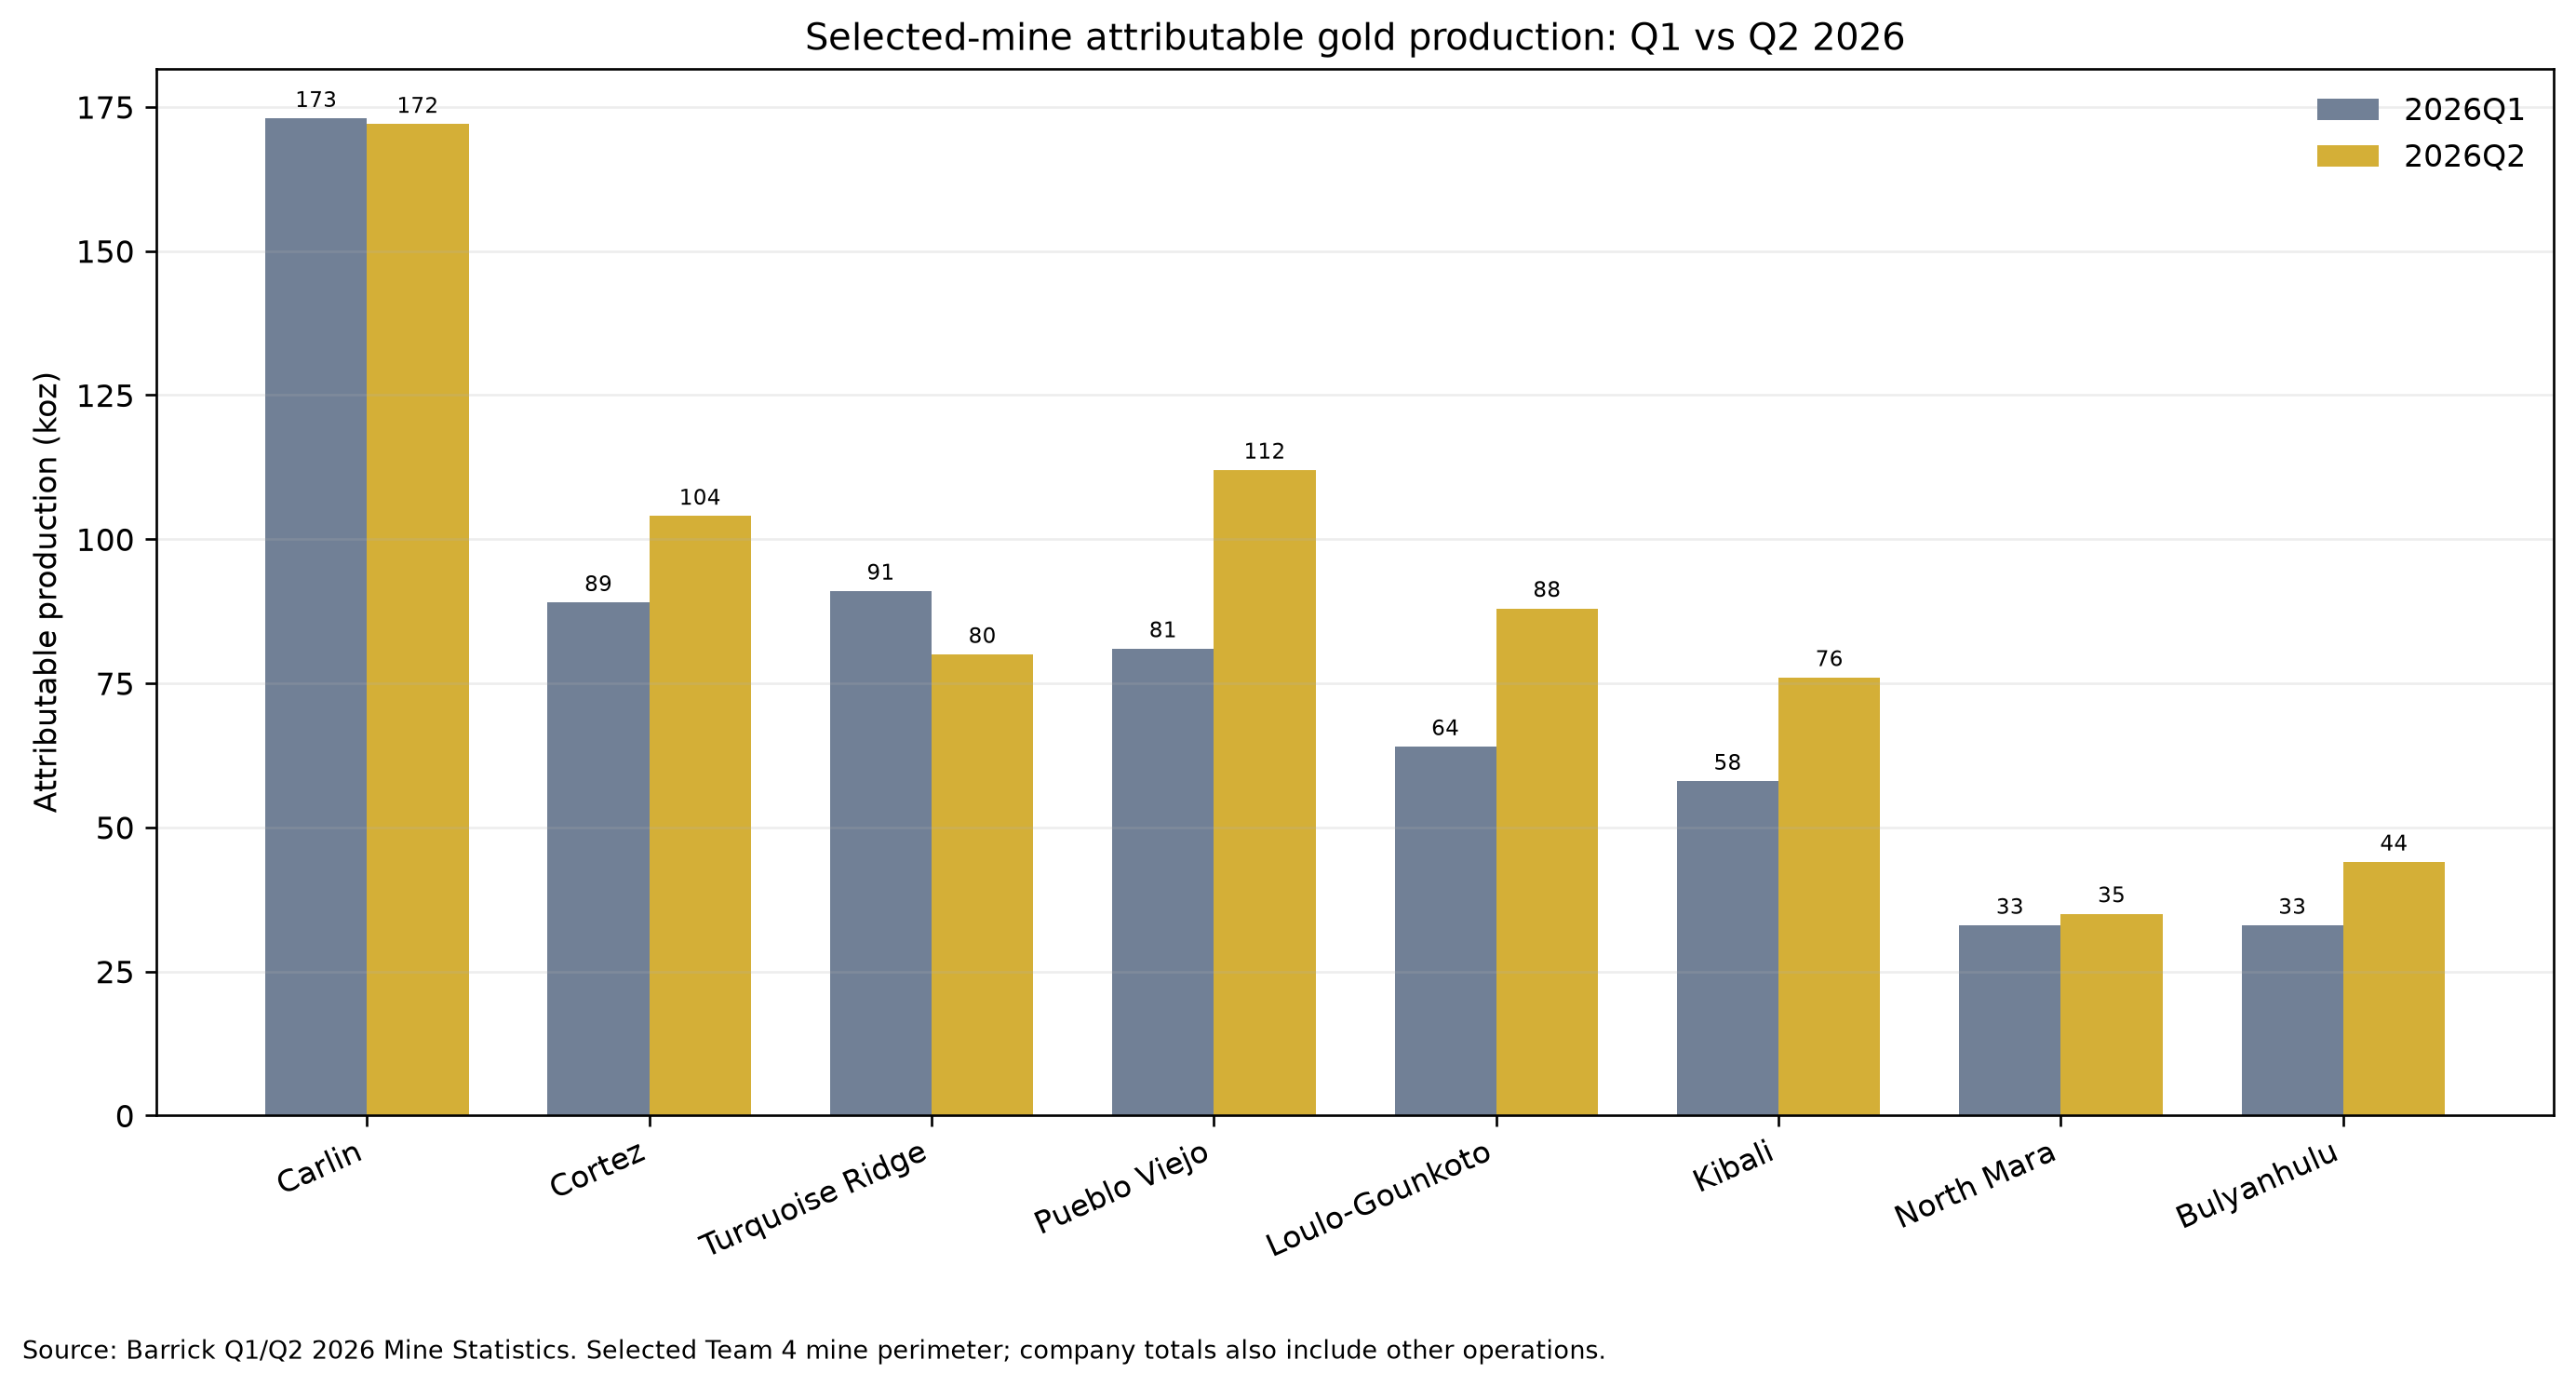
\includegraphics[width=\textwidth]{img/team4_current/team4_mine_production_qoq.png}
    \caption{Attributable gold production for the eight mines retained from
    the Team~4 study, refreshed from Barrick's Q1 and Q2 2026 Mine Statistics.
    These bars are current observations, not simulated production paths.}
    \label{fig:team4-production-qoq}
\end{figure}

\begin{figure}[htbp]
    \centering
    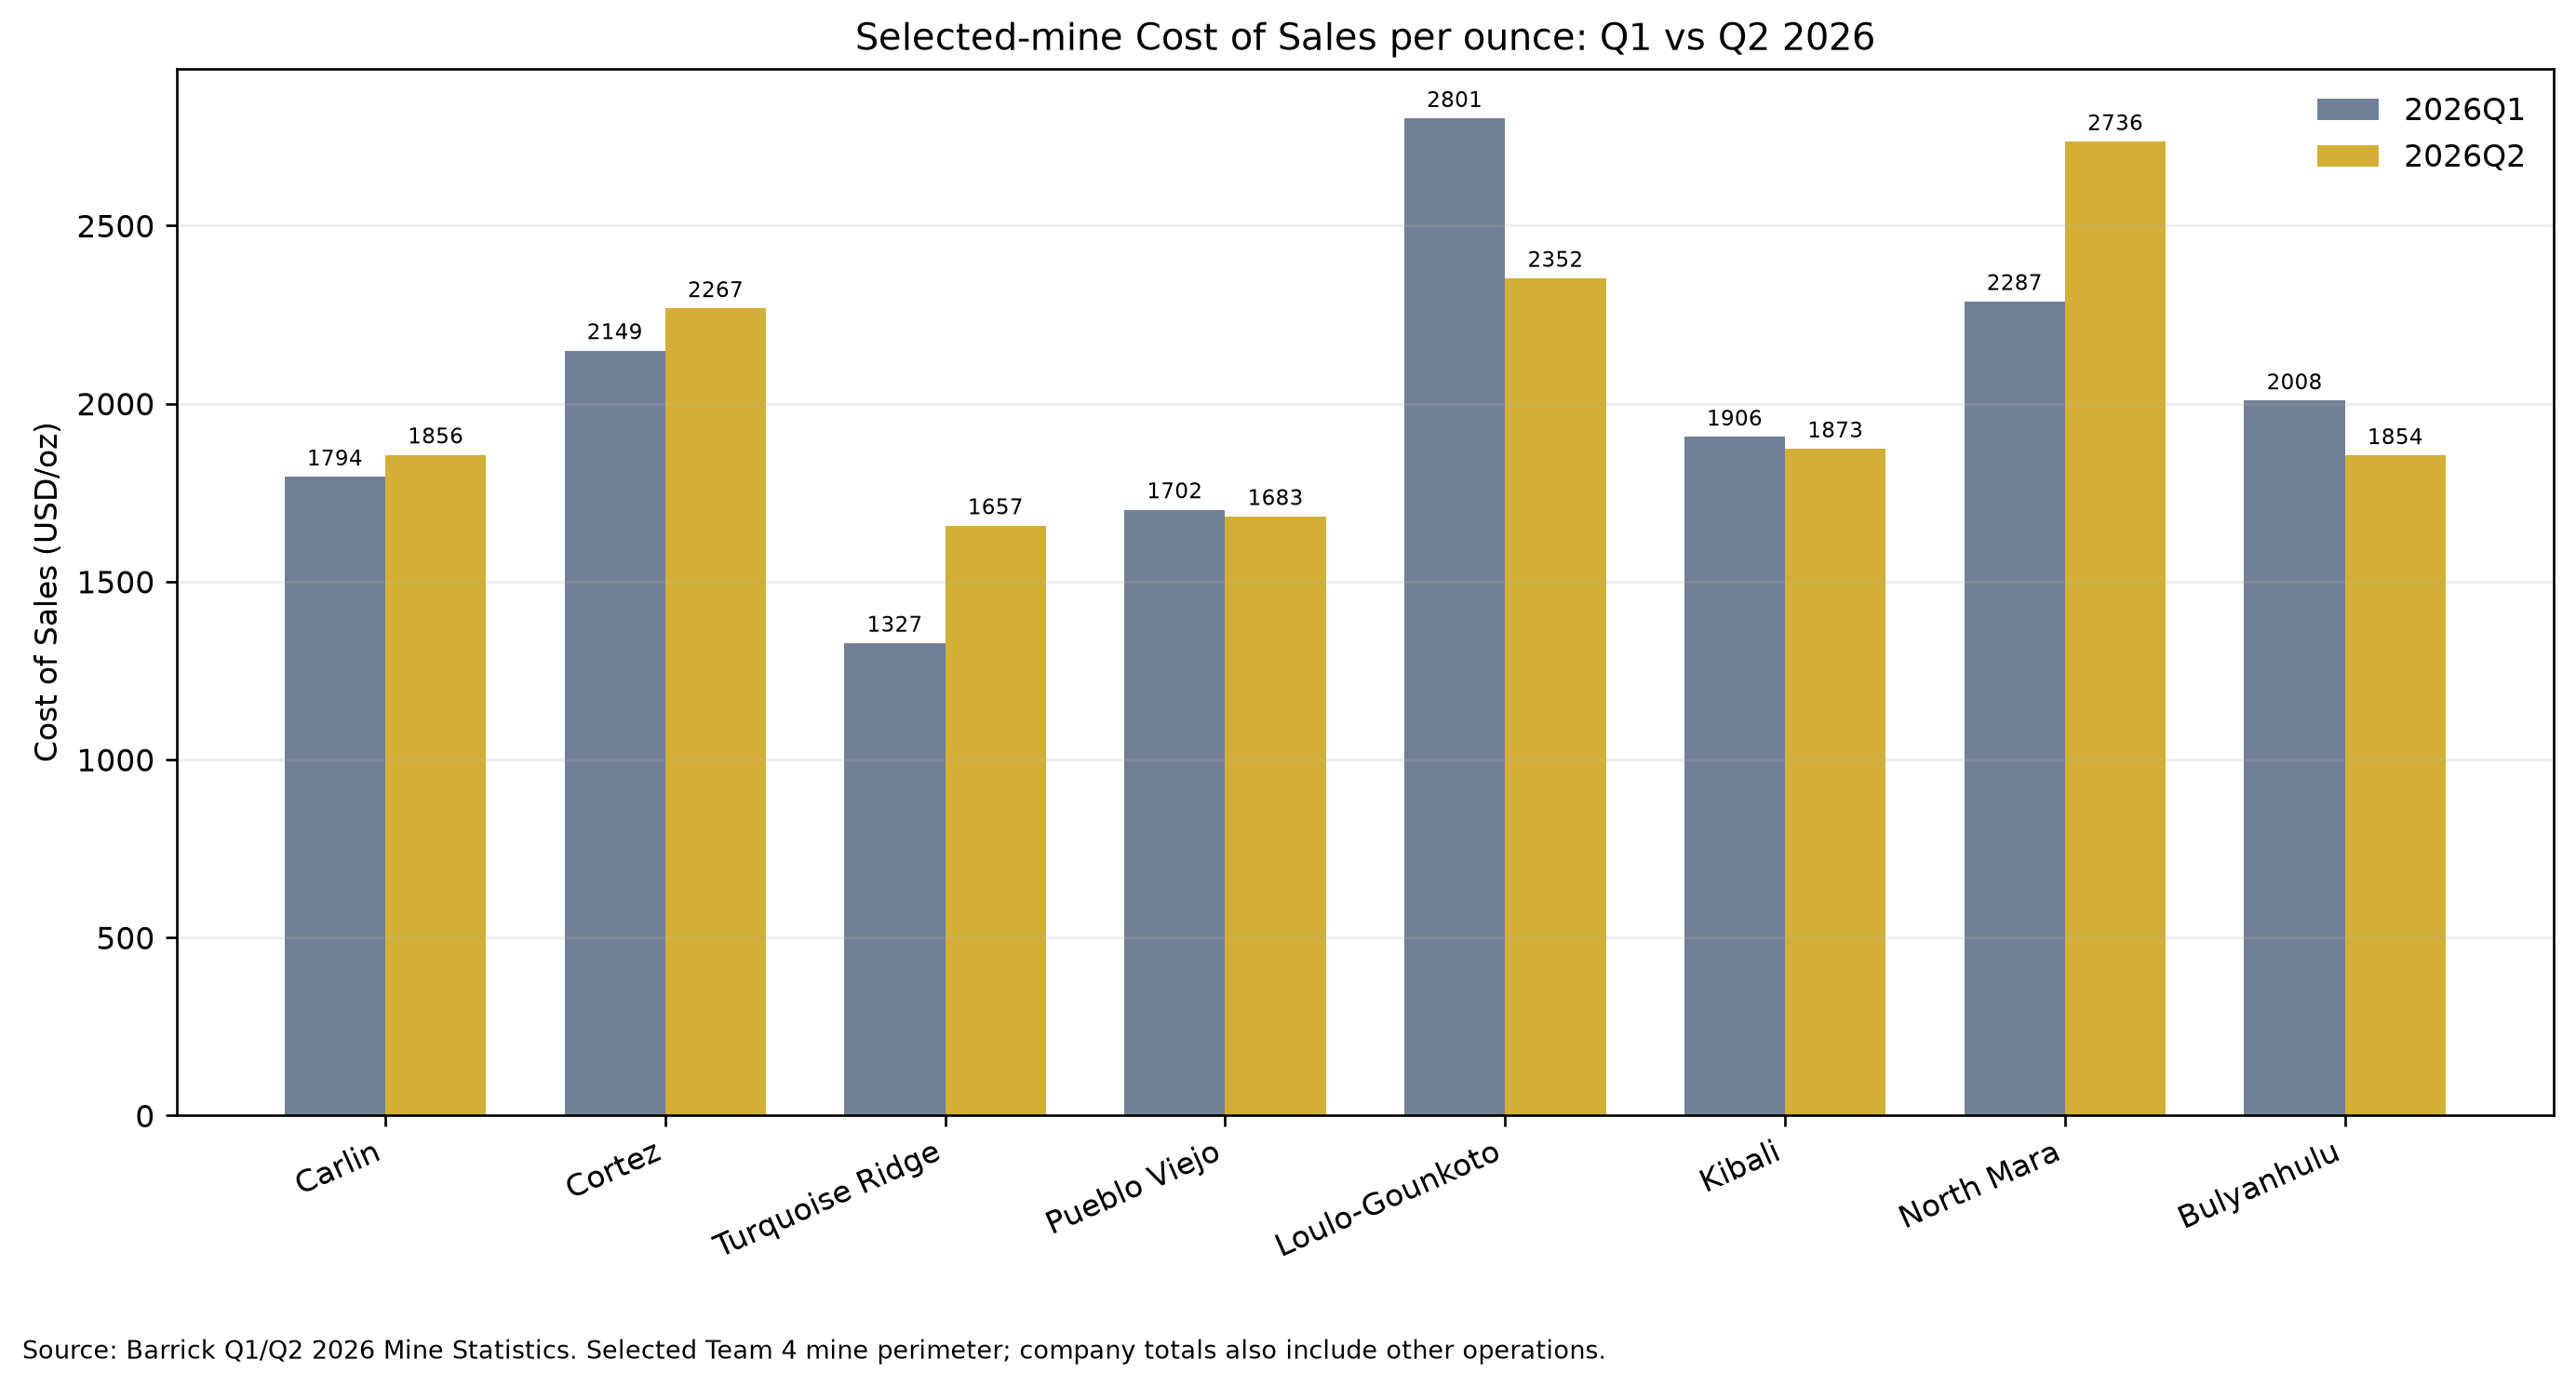
\includegraphics[width=\textwidth]{img/team4_current/team4_mine_cost_qoq.png}
    \caption{Cost of Sales per ounce for the same mine perimeter. The figure
    preserves the Team~4 mine-level comparison while replacing article images
    with a branch-local rendering of current public data.}
    \label{fig:team4-cost-qoq}
\end{figure}

The physical drivers behind production are shown separately in
Figure~\ref{fig:team4-process-components}. This matters because tonnes,
grade and recovery can move in opposite directions: a production change
cannot be interpreted as a price effect, and none of these panels contains a
gold-price input.

\begin{figure}[p]
    \centering
    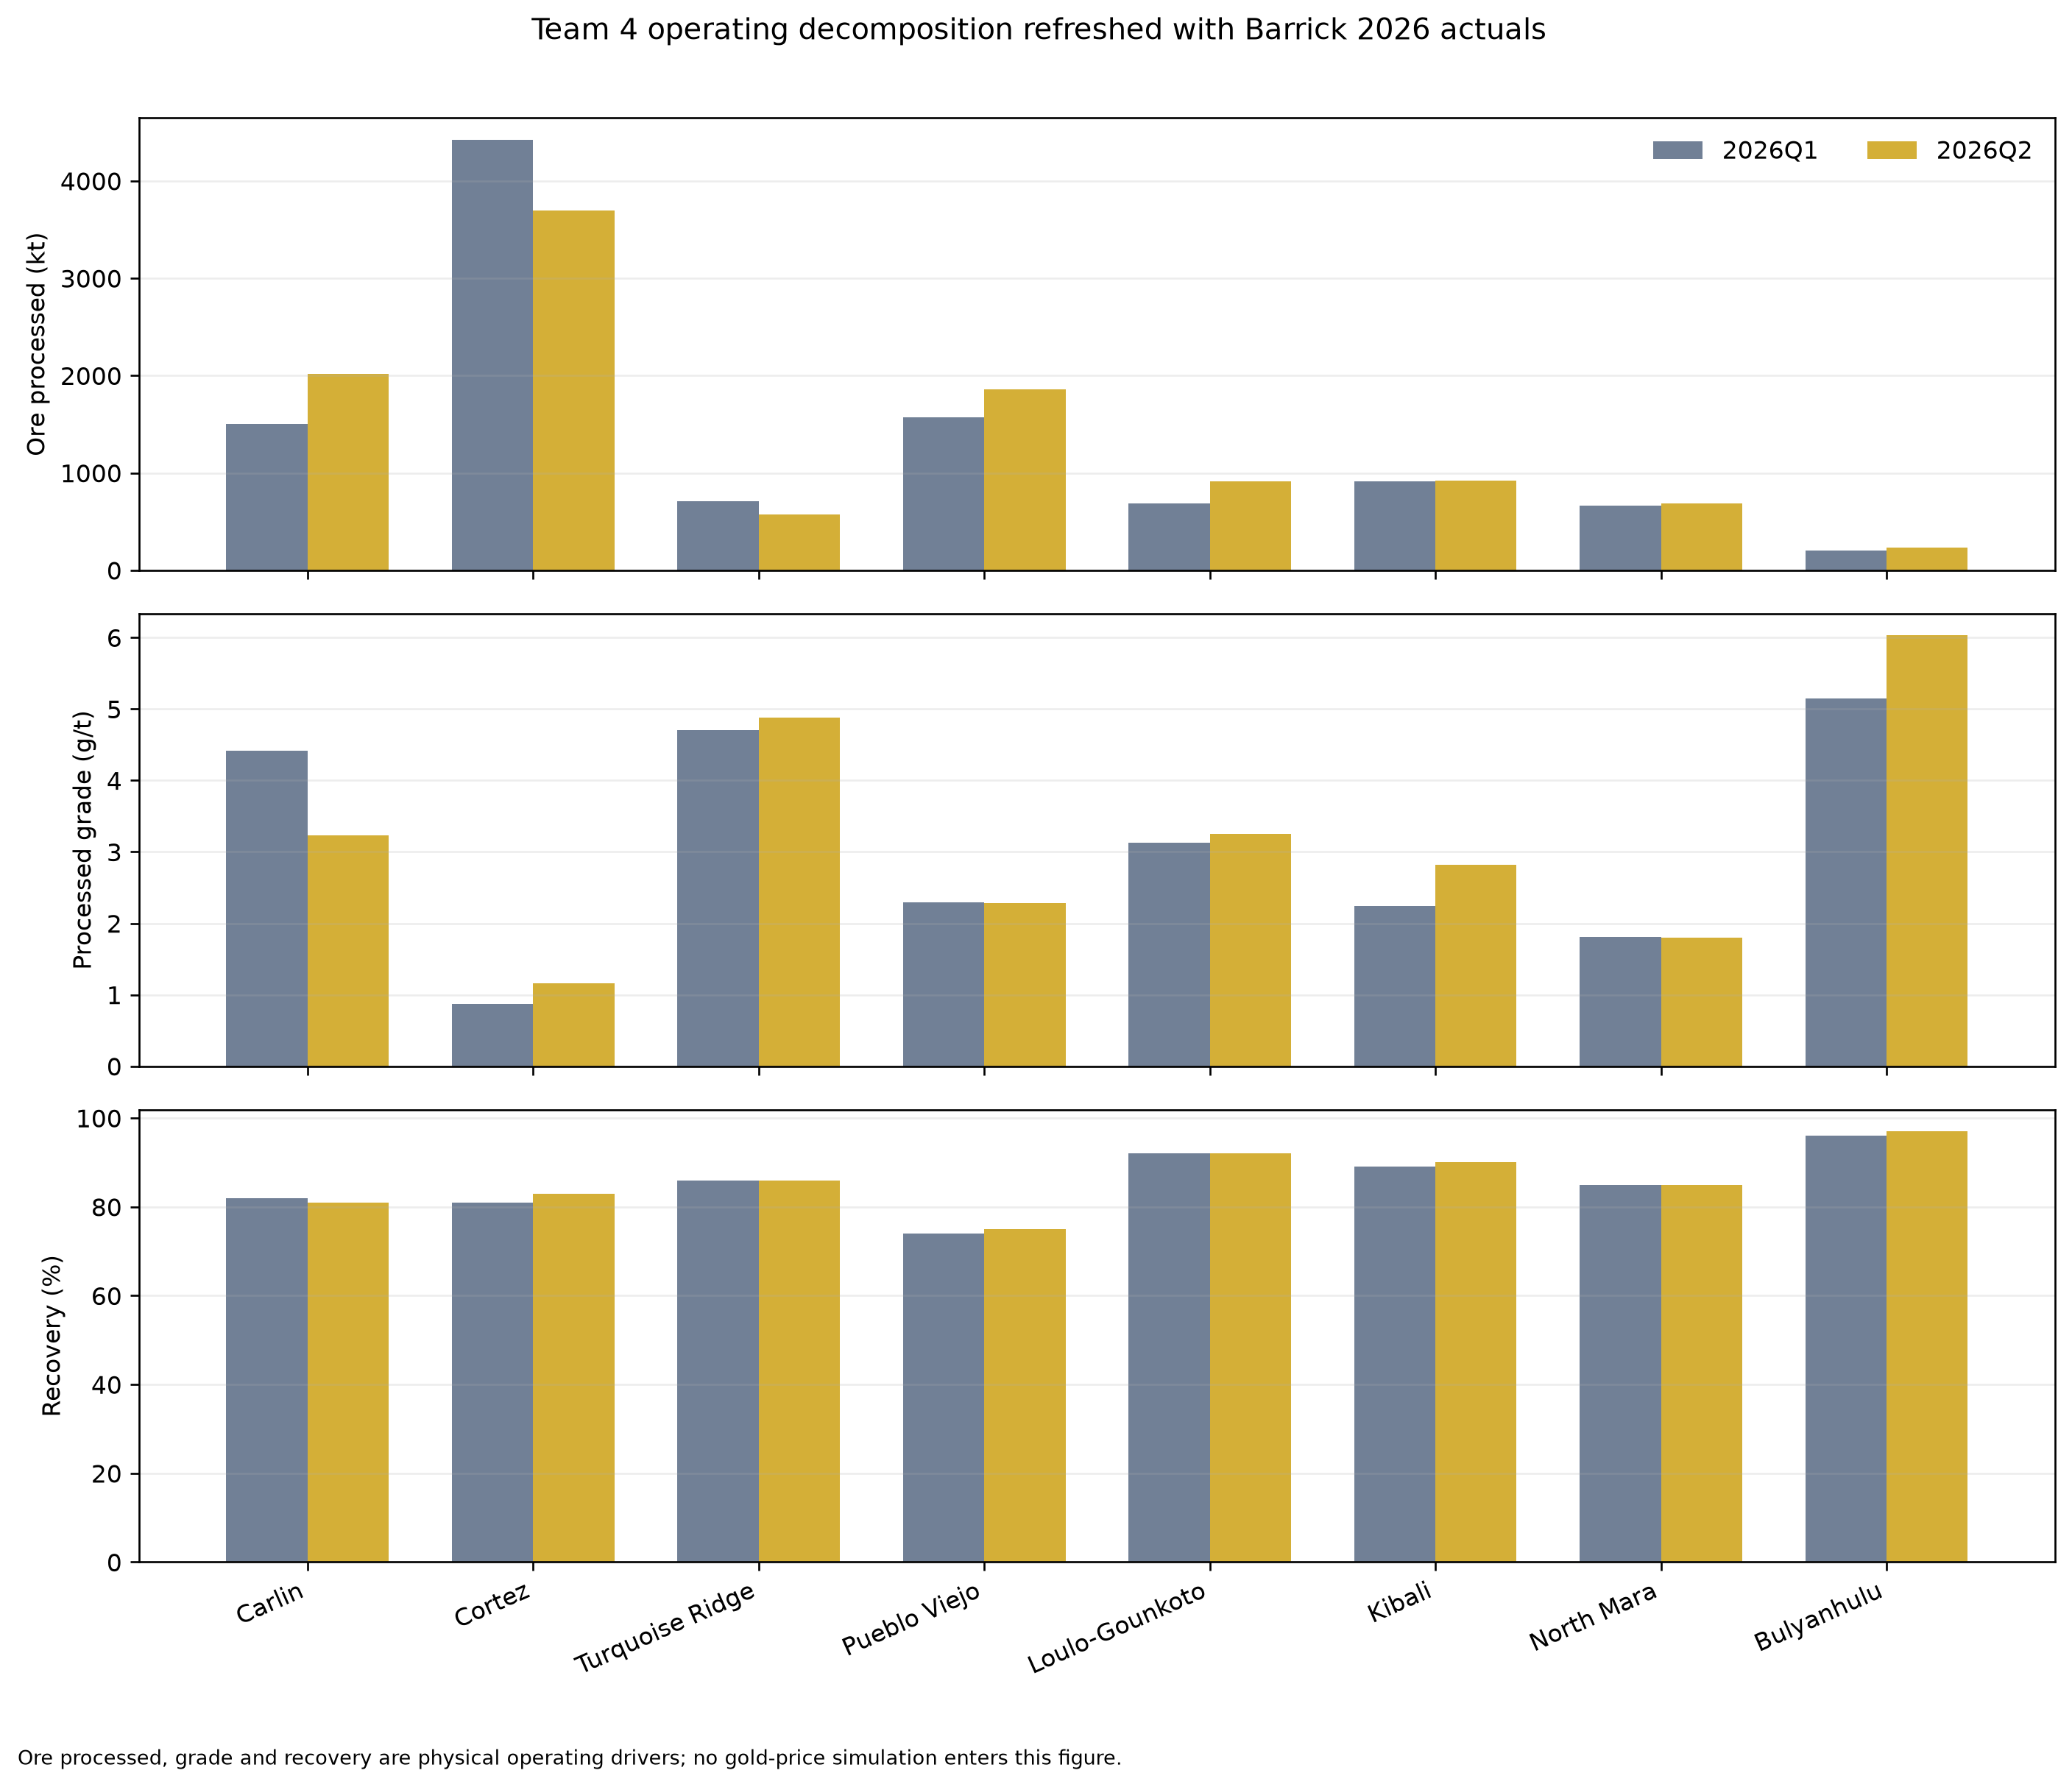
\includegraphics[width=\textwidth]{img/team4_current/team4_process_components_qoq.png}
    \caption{Ore processed, processed grade and recovery in Q1 and Q2 2026.
    Values are transcribed from Barrick's published mine-statistics tables and
    generated by code in this branch.}
    \label{fig:team4-process-components}
\end{figure}

The DCF horizon needs a complete 20-quarter operating vector. The clean
handoff is therefore mixed but explicit: 2026Q1--Q2 are Barrick actuals,
whereas 2026Q3--2030 retain the Team~4 forecasts. Figure~
\ref{fig:team4-operating-contract} marks the boundary in both code and
graphics. This avoids describing a forecast as observed evidence and prevents
the Team~4 price demonstrator from entering the valuation by association.

\begin{figure}[htbp]
    \centering
    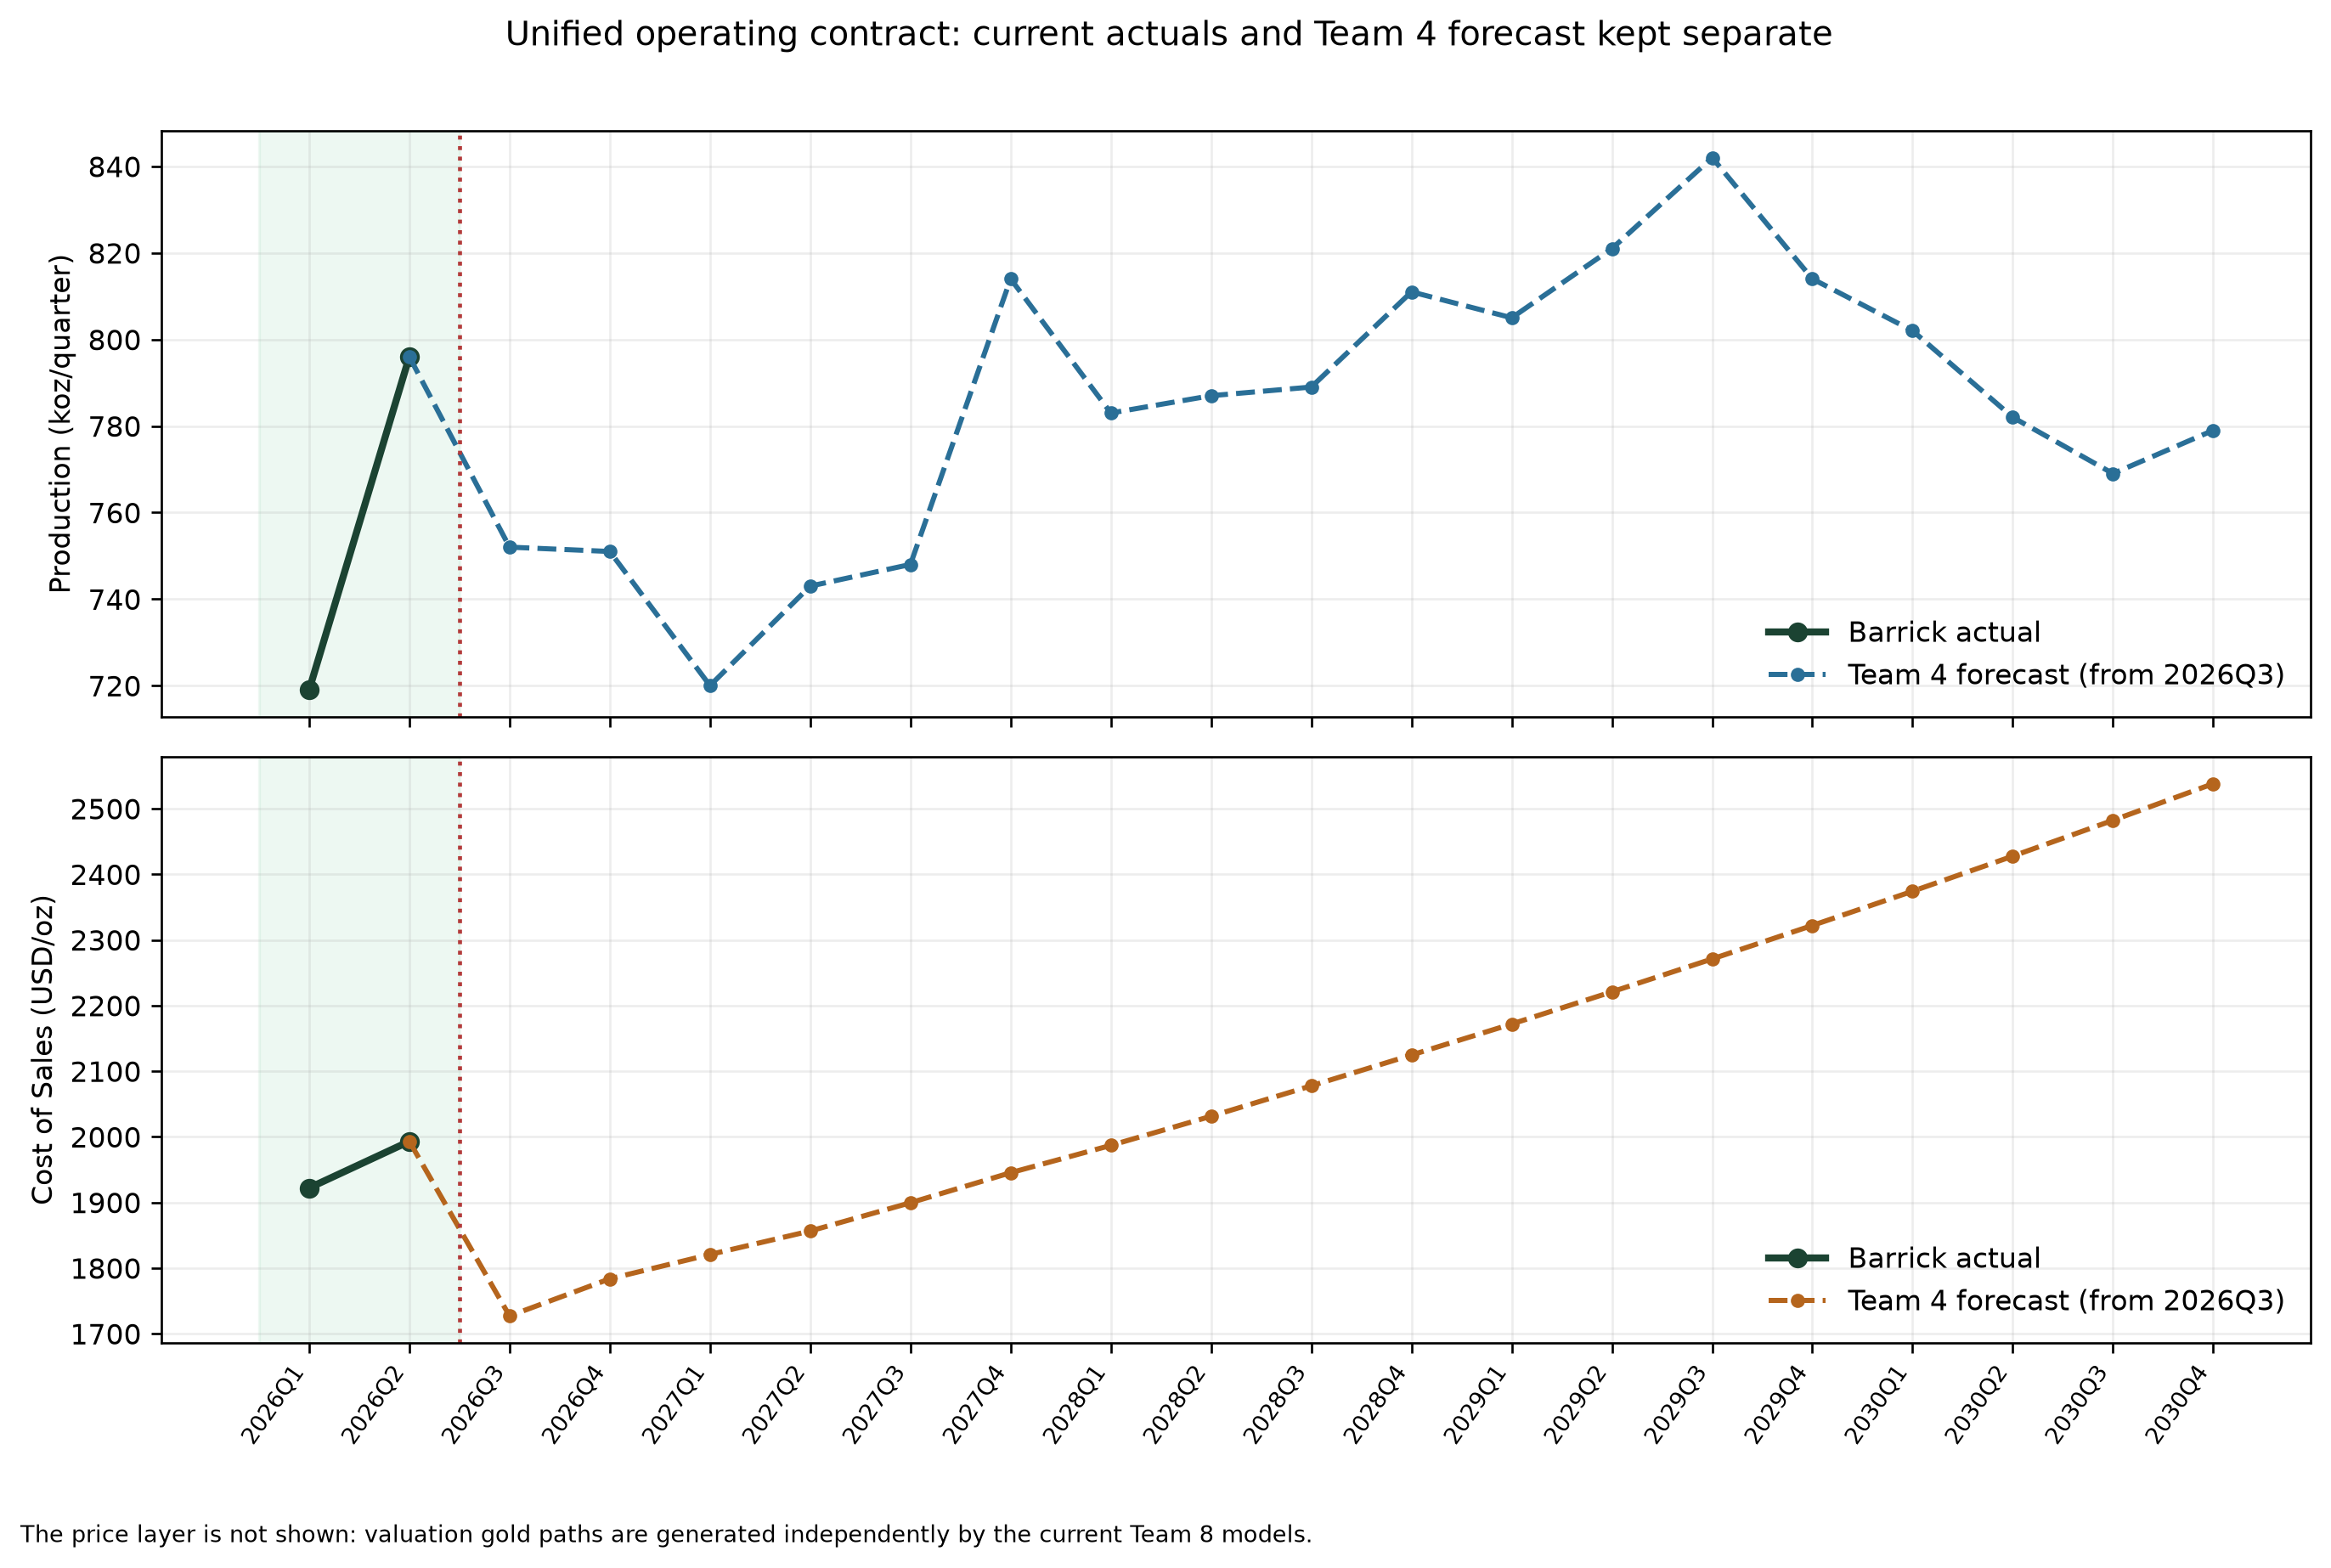
\includegraphics[width=\textwidth]{img/team4_current/team4_operating_contract.png}
    \caption{Operating contract consumed by the unified valuation. Green
    observations are current Barrick actuals; dashed values from 2026Q3 onward
    are Team~4 forecasts. The price layer is absent by design and is supplied
    independently by the current Team~8 models in Chapter~9.}
    \label{fig:team4-operating-contract}
\end{figure}

The remaining operating limitation is economic rather than procedural. The
forecast does not yet model reserves, mine closures, grade-dependent
management actions or endogenous production responses to adverse gold-price
states. Those items remain within the validation boundary and the genuinely
open research agenda; constructing a richer price model is no longer a
Team~4 ``next step'', because that work is already performed in Chapters~8--9.
